\documentclass[12pt,a4paper]{article}

\usepackage[utf8]{inputenc}
\usepackage[T1]{fontenc}
\usepackage[french]{babel}
\usepackage{graphicx}
\usepackage{amsmath, amssymb}
\usepackage{listings}
\usepackage{xcolor}
\usepackage{geometry}
\usepackage{float}
\usepackage{tikz}

\geometry{margin=2.5cm}

\lstset{
    language=Python,
    basicstyle=\ttfamily\small,
    frame=single,
    breaklines=true,
    showstringspaces=false
}

\title{TP OST -- Décision dans l'incertain \& Sécurité \\ Compte rendu}
\author{NOM Prénom}  % <-- A REMPLACER
\date{2025--2026}

\begin{document}
\maketitle

% ============================================================
\section{Code source et exécution}
% ============================================================

Fichiers :
\begin{itemize}
    \item \texttt{environment.py} -- environnement Bernoulli + fonction \texttt{pull(i)}
    \item \texttt{algorithmes\_A.py} -- les 4 algorithmes (Random, $\varepsilon$-greedy, $\varepsilon$-greedy-dec, UCB)
    \item \texttt{bandit.py} -- cadre générique (Figure~1)
    \item \texttt{question1.py}, \texttt{question2.py}, \texttt{question3.py} -- scripts par question
    \item \texttt{partie2.py} -- protocole sécurisé (Partie 2)
    \item \texttt{main.py} -- point d'entrée
\end{itemize}

\begin{lstlisting}[language=bash]
source venv/bin/activate
python3 main.py 1     # Question 1
python3 main.py 2     # Question 2
python3 main.py 3     # Question 3
python3 main.py p2    # Partie 2
\end{lstlisting}

% ============================================================
\section{Partie 1 -- Implémentation et comparaison}
% ============================================================

% ------------------------------------------------------------
\subsection{Question 1 -- Implémentation}
% ------------------------------------------------------------

On a implémenté les 4 algorithmes de la Figure~2 dans le cadre générique de la Figure~1. Pour vérifier que tout marche, on lance avec $K=4$ bras, $\mu = [0.2, 0.4, 0.6, 0.8]$, $N=10000$ :

% Collez ici la vraie sortie de python3 main.py 1 :
\begin{verbatim}
  random          : cumulative reward = ...
  e-greedy        : cumulative reward = ...
  e-greedy-dec    : cumulative reward = ...
  UCB             : cumulative reward = ...
\end{verbatim}

On voit que random tourne autour de 5000 ($= \bar{\mu} \times N$) et UCB est proche de 8000 ($= \mu^* \times N$), donc les algorithmes fonctionnent comme prévu.

% ------------------------------------------------------------
\subsection{Question 2 -- Benchmark}
% ------------------------------------------------------------

On a lancé les 4 algorithmes avec $K=5$, $\mu = [0.1, 0.2, 0.3, 0.4, 0.5]$, pour $N$ allant de $10^5$ à $10^6$. Chaque point est la moyenne de 100 runs.

\begin{figure}[H]
    \centering
    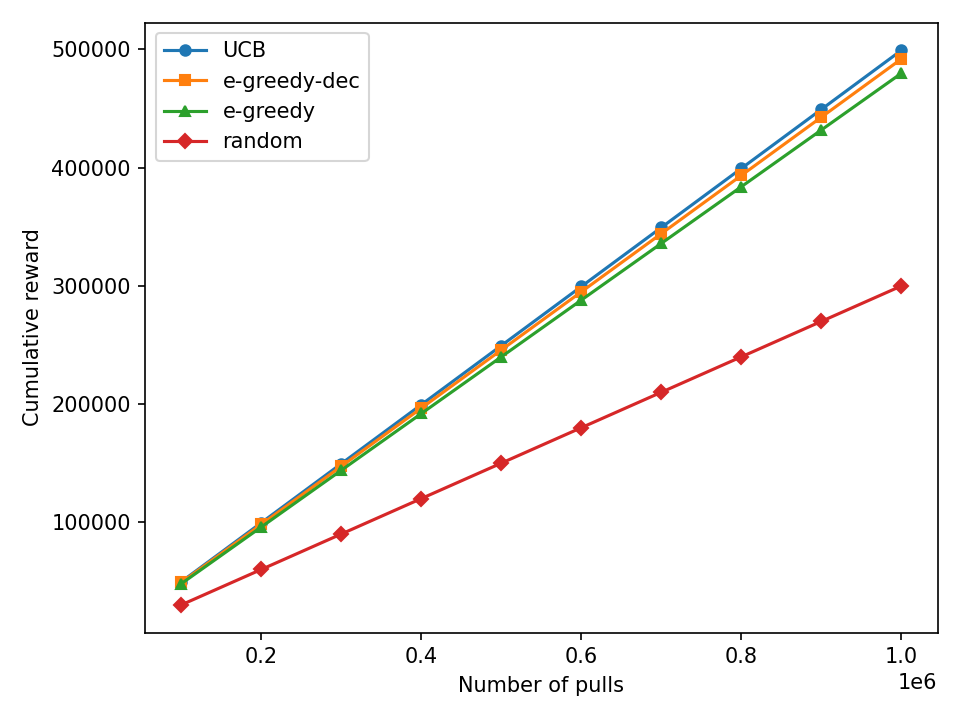
\includegraphics[width=0.8\textwidth]{figures/q2_cumulative_reward.png}
    \caption{Cumulative reward en fonction du nombre de pulls.}
    \label{fig:q2_reward}
\end{figure}

\begin{figure}[H]
    \centering
    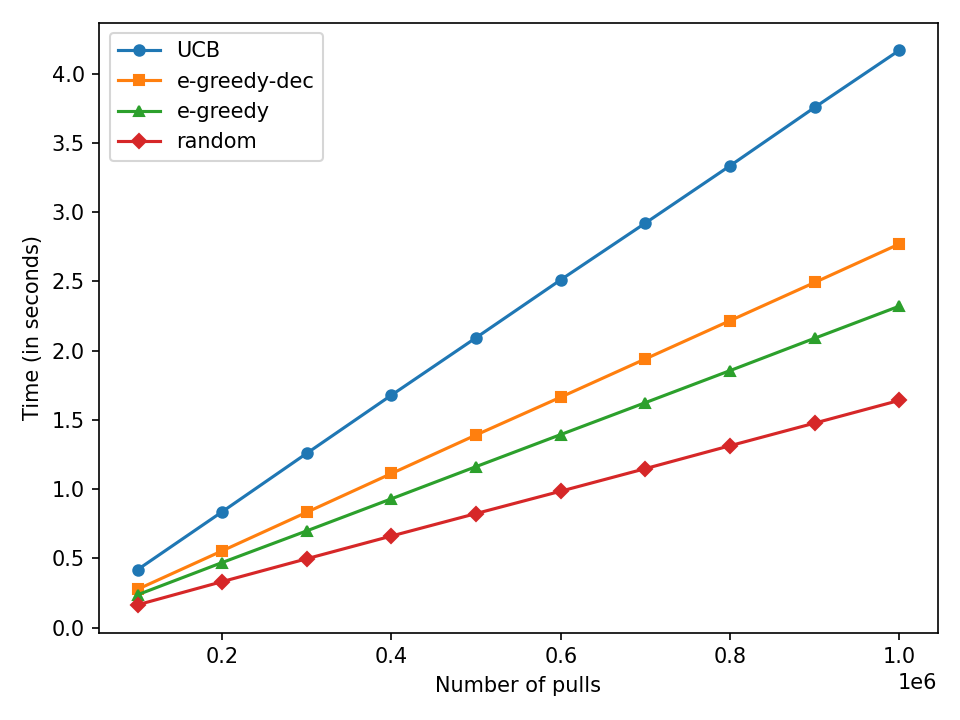
\includegraphics[width=0.8\textwidth]{figures/q2_time.png}
    \caption{Temps d'exécution en fonction du nombre de pulls.}
    \label{fig:q2_time}
\end{figure}

Sur la Figure~\ref{fig:q2_reward}, UCB donne le meilleur reward (proche de $\mu^* \times N = 500\,000$), random est en bas (autour de $300\,000 = \bar{\mu} \times N$), et les deux e-greedy sont entre les deux. e-greedy-dec fait un peu mieux que e-greedy fixe parce que son $\varepsilon$ diminue : il finit par exploiter plus. Avec e-greedy fixe, on gaspille toujours 10\% des pulls en exploration.

Sur la Figure~\ref{fig:q2_time}, UCB est le plus lent parce qu'il calcule un \texttt{sqrt} et un \texttt{log} pour chaque bras à chaque pas. e-greedy-dec est un peu plus lent que e-greedy fixe à cause du calcul de $\varepsilon = 1/\ln(t^2)$. Random est le plus rapide, il tire juste un bras au hasard.

% ------------------------------------------------------------
\subsection{Question 3 -- Deux scénarios}
% ------------------------------------------------------------

On teste deux scénarios différents pour voir comment les algorithmes réagissent quand les $\mu$ changent.

\subsubsection{Scénario A : $\mu = [0.1, 0.3, 0.5, 0.7, 0.9]$}

Les bras sont bien séparés, le meilleur est à $\mu^* = 0.9$.

\begin{figure}[H]
    \centering
    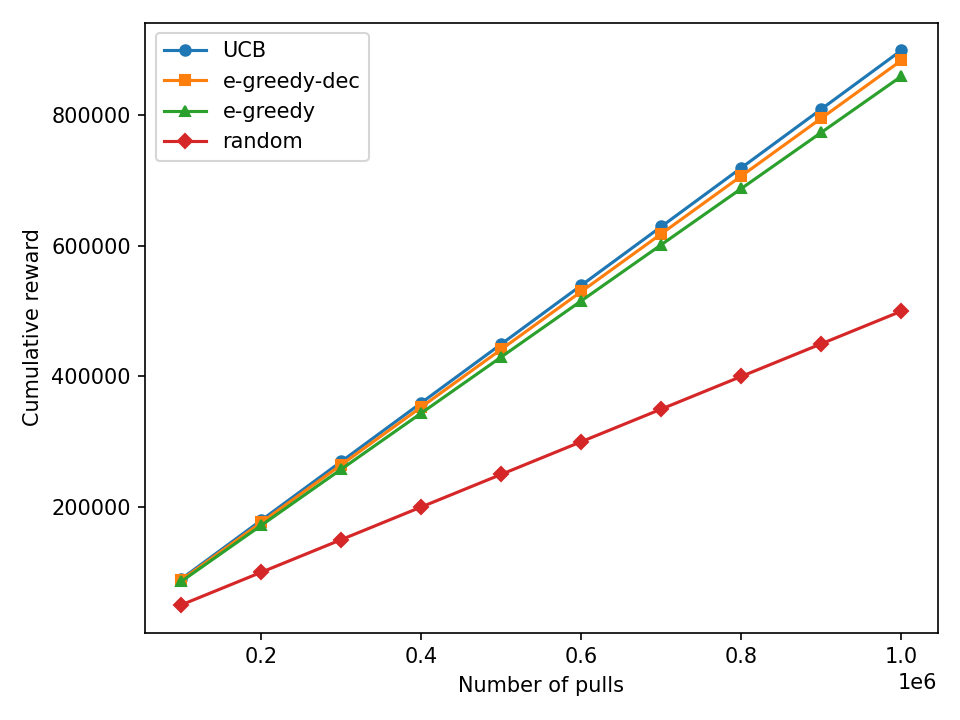
\includegraphics[width=0.8\textwidth]{figures/q3a_cumulative_reward.png}
    \caption{Cumulative reward -- Scénario A.}
    \label{fig:q3a_reward}
\end{figure}

\begin{figure}[H]
    \centering
    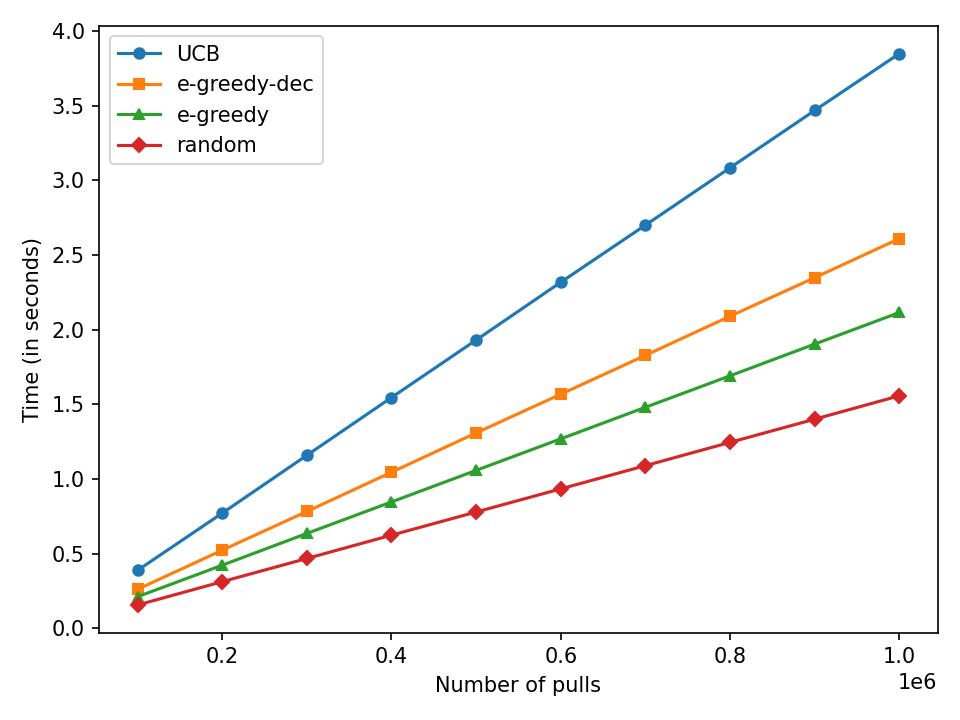
\includegraphics[width=0.8\textwidth]{figures/q3a_time.png}
    \caption{Temps d'exécution -- Scénario A.}
    \label{fig:q3a_time}
\end{figure}

UCB atteint $\approx 895\,000$ (proche de $\mu^* \times N$), random $\approx 500\,000$ ($= \bar{\mu} \times N$). L'écart est grand : UCB fait presque le double de random. Les e-greedy sont entre les deux, et e-greedy-dec fait un peu mieux que e-greedy fixe car son $\varepsilon$ diminue avec le temps. Pour le temps, UCB est environ 2x plus lent que random ($\approx 3.8$s vs $\approx 1.6$s).

\subsubsection{Scénario B : $\mu = [0.78, 0.80, 0.82, 0.84, 0.86]$}

Les bras sont très proches, l'écart entre le pire et le meilleur est seulement de 0.08.

\begin{figure}[H]
    \centering
    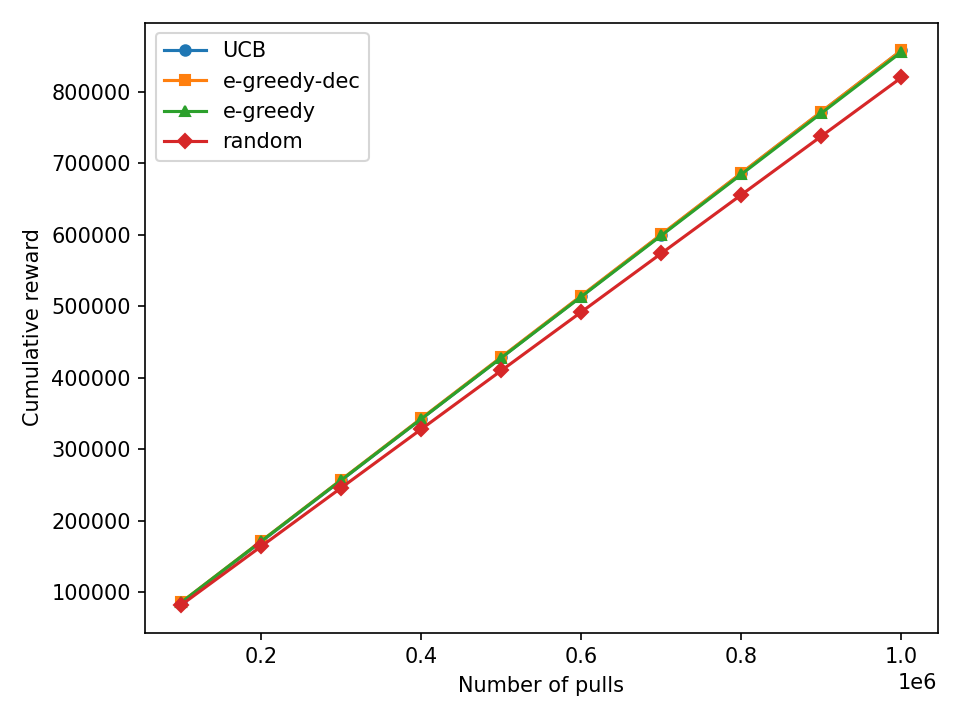
\includegraphics[width=0.8\textwidth]{figures/q3b_cumulative_reward.png}
    \caption{Cumulative reward -- Scénario B.}
    \label{fig:q3b_reward}
\end{figure}

\begin{figure}[H]
    \centering
    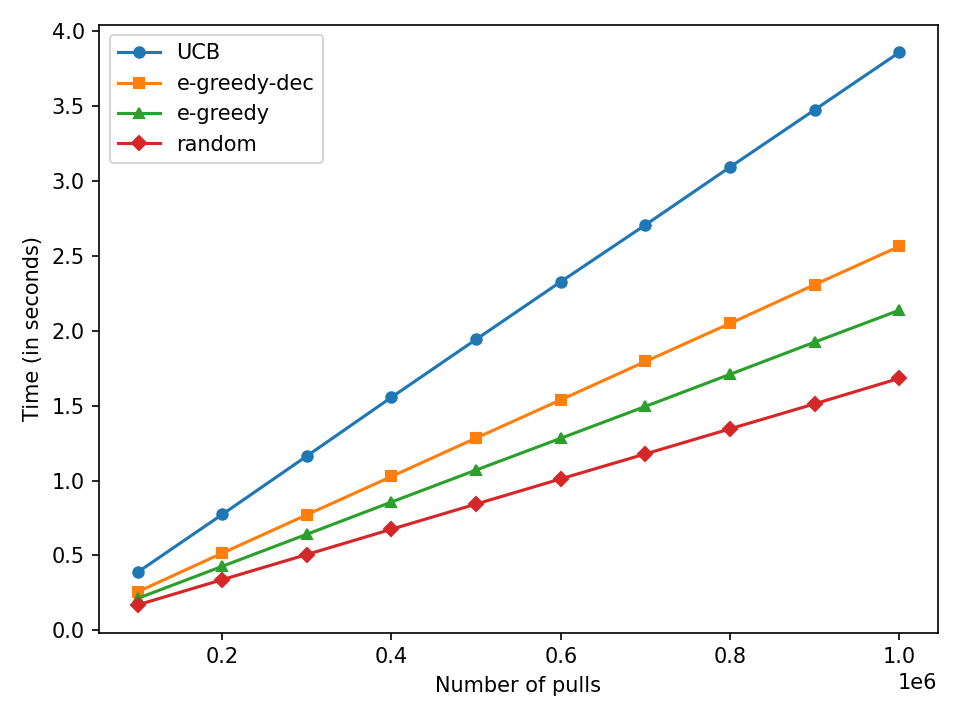
\includegraphics[width=0.8\textwidth]{figures/q3b_time.png}
    \caption{Temps d'exécution -- Scénario B.}
    \label{fig:q3b_time}
\end{figure}

UCB, e-greedy-dec et e-greedy sont presque superposés ($\approx 855\,000$). Random est juste en dessous ($\approx 820\,000 = \bar{\mu} \times N$). L'écart max n'est que de $35\,000$, contre $395\,000$ dans le scénario A. Comme les bras se valent, même tirer au hasard donne un bon score. Du coup les e-greedy font aussi bien que UCB en reward, mais pour $\approx 2$s contre $\approx 3.8$s (Figure~\ref{fig:q3b_time}).

\subsubsection{Bilan}

Bras différents $\to$ UCB a un vrai avantage en reward. Bras proches $\to$ e-greedy suffit et coûte moins cher en temps. UCB est toujours le plus lent quel que soit le scénario, donc le choix dépend de la situation : si on s'attend à des bras très différents, UCB vaut le coup ; sinon, un e-greedy est plus raisonnable.

% ============================================================
\section{Partie 2 -- Protocole sécurisé}
% ============================================================

\subsection{Contexte}

Dans un scénario MLaaS (Machine Learning as a Service), un client veut exécuter un algorithme de bandit mais délègue le calcul à un serveur cloud. Le souci, c'est que le serveur voit les rewards à chaque étape.

Si les rewards sont sensibles (résultats médicaux, clics utilisateurs, etc.), on ne veut pas qu'un serveur seul puisse les lire. C'est ce problème qu'on essaie de résoudre ici, en s'inspirant des travaux présentés en cours sur les protocoles sécurisés pour bandits.

\subsection{Application}

Un hôpital teste $K$ traitements sur des patients. À chaque étape, il donne un traitement (= pull d'un bras) et observe si le patient va mieux ($r = 1$) ou non ($r = 0$). L'hôpital veut utiliser UCB pour trouver le meilleur traitement, mais il externalise le calcul à deux serveurs cloud. Les données patients ne doivent pas être exposées.

Un attaquant qui contrôle un des serveurs pourrait sinon reconstituer l'historique médical des patients : quel traitement a marché pour qui.

\subsection{Modèle de sécurité}

\begin{itemize}
    \item \textbf{Participants} : 1 client (hôpital), 2 serveurs cloud
    \item \textbf{Adversaire} : semi-honnête (honest-but-curious) -- chaque serveur suit le protocole mais essaie de déduire les rewards
    \item \textbf{Garantie} : tant que les 2 serveurs ne coopèrent pas, aucun ne peut reconstituer les vrais rewards
    \item \textbf{Hypothèse} : les serveurs sont hébergés par des fournisseurs indépendants (par ex. AWS et OVH)
\end{itemize}

\subsection{Protocole : UCB + secret sharing additif}

L'idée est simple : au lieu d'envoyer le reward $r$ en clair, le client le coupe en 2 parts aléatoires $r_1, r_2$ telles que $r_1 + r_2 = r$. Il envoie $r_1$ au serveur 1, $r_2$ au serveur 2. Chaque serveur ne voit qu'un nombre aléatoire.

\textbf{Initialisation :} pour chaque bras $i \in \{1, \ldots, K\}$, le client tire $r = \text{pull}(i)$, génère $r_1 \leftarrow \text{aléatoire}$, pose $r_2 = r - r_1$, et envoie les parts aux serveurs. Chaque serveur $j$ initialise $s^{(j)}_i = r_j$, $n_i = 1$.

\textbf{À chaque tour $t$ :}
\begin{enumerate}
    \item Les 2 serveurs calculent conjointement les scores UCB :
    $$\text{score}_i = \frac{s^{(1)}_i + s^{(2)}_i}{n_i} + \sqrt{\frac{2 \ln t}{n_i}}$$
    Chacun a une part de $s_i$. Ils combinent via un calcul sécurisé (MPC) sans révéler leurs parts respectives.
    \item Le bras $i_m$ avec le meilleur score est envoyé au client.
    \item Le client tire $r = \text{pull}(i_m)$.
    \item Le client génère $r_1 \leftarrow \text{aléatoire}$, $r_2 = r - r_1$.
    \item Envoie $r_1$ à Serveur 1, $r_2$ à Serveur 2.
    \item Chaque serveur met à jour : $s^{(j)}_{i_m} \mathrel{+}= r_j$, $n_{i_m} \mathrel{+}= 1$.
\end{enumerate}

\subsection{Messages échangés}

\begin{figure}[H]
\centering
\begin{tikzpicture}
    \node[font=\bfseries] at (0,0) {Client};
    \node[font=\bfseries] at (4,0) {Serveur 1};
    \node[font=\bfseries] at (8,0) {Serveur 2};

    \draw[dashed] (0,-0.4) -- (0,-6);
    \draw[dashed] (4,-0.4) -- (4,-6);
    \draw[dashed] (8,-0.4) -- (8,-6);

    \draw[->,thick] (0,-1.2) -- node[above,font=\footnotesize] {$r_1$ (aléatoire)} (3.8,-1.6);
    \draw[->,thick] (0,-1.2) -- node[above,font=\footnotesize,yshift=4pt] {$r_2 = r - r_1$} (7.8,-1.6);

    \draw[<->,thick] (4,-2.8) -- node[above,font=\footnotesize] {calcul conjoint UCB (MPC)} (8,-2.8);

    \draw[<-,thick] (0.2,-4) -- node[above,font=\footnotesize] {bras choisi $i_m$} (3.8,-4);

    \node[font=\footnotesize] at (0,-5) {$r = \text{pull}(i_m)$};
    \node[font=\footnotesize,gray] at (4,-5.5) {(répéter $N$ fois)};
\end{tikzpicture}
\caption{Échange de messages à chaque tour.}
\label{fig:protocol}
\end{figure}

\subsection{Vérification}

Le fichier \texttt{partie2.py} simule ce protocole. On compare le reward cumulé avec UCB classique : les deux donnent le même résultat, car les parts s'annulent ($r_1 + r_2 = r$). On affiche aussi ce que chaque serveur voit pour un bras donné : des valeurs aléatoires, inutilisables seules.

\begin{lstlisting}[language=bash]
python3 main.py p2
\end{lstlisting}

\subsection{Limites}

\begin{itemize}
    \item Si les 2 serveurs coopèrent, ils reconstituent les rewards. Il faut des fournisseurs indépendants.
    \item La communication est doublée (2 messages par reward au lieu de 1).
    \item Le calcul conjoint du score UCB via MPC ajoute de la latence, mais les opérations restent simples (additions, comparaisons).
    \item On pourrait renforcer le protocole avec du secret sharing à seuil (Shamir) pour plus de serveurs, mais 2 suffisent pour notre cas.
\end{itemize}

\end{document}
